\begin{partbacktext}
\part{Aplicaciones}

\end{partbacktext}
%\chapauthor{Autor}
%\chapsubtitle{Subtítulo}
\chapter{Bifurcación de la ecuación logística}\index{Ecuación logística}
\abstract{Muchas aplicaciones involucran problemas inversos. En esta sección, }
%\chaptermark{xd}
\section{Ecuación diferencial ordinaria lineal}

\begin{pylabcode}[plotsession]
rc('text', usetex=True)
rc('font', **{'family':'serif', 'serif':['Times']})
rc('legend', fontsize=10.0)
x = linspace(0,3*pi)
figure(figsize=(3.25,2))
plot(x, sin(x), label='$\sin x$')
plot(x, sin(x)**2, label='$\sin^{2}(x)$',linestyle='dashed')
xlabel(r'$x$-axis')
ylabel(r'$y$-axis')
xticks(arange(0,4*pi, pi), ('$0$', '$\pi$', '$2\pi$', '$3\pi$'))
axis([0, 3*pi, -1, 1])
legend(loc='lower right')
savefig('img/myplot.pdf', bbox_inches='tight')
\end{pylabcode}

\begin{figure}
	\centering
	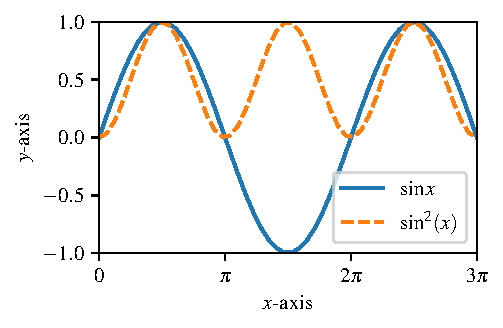
\includegraphics{./img/myplot}
	\caption{\label{fig:matlpotlib} A plot created with PythonTeX}
\end{figure}